\chapter{拓扑物态的深度学习} \label{sec:topoml}

这一章,我们将介绍利用机器学习方法进行拓扑分类的研究。首先,在5.1节,我们来回顾无相互作用费米子波函数的拓扑分类问题,着重分析无对称性以及被手性对称性保护的绝缘体系统。为了让机器习得这些系统的拓扑分类,我们采取了卷积神经网络的方法——在5.2节我们对这一方法进行简单介绍。最后,在5.3与5.4节,我们将会分别将神经网络方法应用于二维陈绝缘体与一维手性对称性保护的体系上,经过训练,我们将看到机器可以对不在训练数据内的全新的哈密顿量的拓扑数进行精确预言。通过将神经网络打开,我们还能直接对其机理进行分析。


\section{拓扑绝缘体分类}
正如前文所述,拓扑绝缘体在近年来受到了广泛的关注。受益于早年间对特殊模型研究的积累,人们逐渐建立起了对有能隙的无相互作用费米子体系拓扑分类\cite{topoclassify2016}的系统性理解:对于任意的$d$维系统,按照其是否存在时间反演对称性$\hat{T}$,粒子空穴对称性$\hat{C}$以及手性对称性$\hat{S}$,我们可以将其分为A,AIII,AI,BDI,D,DIII,AII,CII,C,CI十类,其拓扑分类随$d$变化呈现周期性结构。作为其中最简单的两个例子,A和AIII类不包含任何反厄米对称性,它们被称为复对称类。我们这里主要来考虑这两类拓扑绝缘体。

A类的拓扑绝缘体不存在任何对称性约束。其非平凡的拓扑分类只存在于偶数维度$d=2n$中,这时其分类由陈数$\mathcal{C}_n$给出:
\begin{align}
\mathcal{C}_n&=\frac{1}{n!}\left(\frac{1}{2\pi}\right)^n\int \text{tr}\ \mathcal{F}^n,\\
\mathcal{F}&=d\mathcal{A}-\ii \mathcal{A}^2.
\end{align}
其中类似绝热演化中的定义,$\mathcal{A}$为被填充能带的非阿贝尔联络:
$\mathcal{A}=\mathcal{A}_i^{m n}dk^i=i\left<u^m(\mathbf{k})|\partial_{k_i}|u^n(\mathbf{k})\right>dk^i$,而对应的$\mathcal{F}$则为非阿贝尔曲率。为了简便,我们使用了微分形式的记号。

A类拓扑绝缘体一个重要的例子就是在$n=1$情况下的陈绝缘体,它包含引言中提到的的Hofstadter-Harper模型与Haldane 模型。这时,系统的拓扑分类由第一陈数$\mathcal{C}$给出:
\begin{align}
\mathcal{C}&=\left(\frac{1}{2\pi}\right)\int \text{tr}\ \mathcal{F}=\left(\frac{1}{2\pi}\right)\int dk_x dk_y \sum_n F_{xy}^n.
\end{align}
其中$F^n_{xy}$为第$n$个被填充能态的Berry曲率。注意到上式与\eqref{Chern}的一致性,因此本质上二维陈绝缘体与一维系统的的拓扑电子泵现象相一致。在本章第三节,我们将训练深度神经网络,教会机器对这一二维材料进行拓扑分类。

与A类绝缘体不同,AIII类绝缘体存在手性对称性保护。在一次量子化框架下,这要求存在幺正矩阵$U_S$满足:
\begin{align}
U_SH(\mathbf{k})U_S^\dagger=-H(\mathbf{k}).\label{Scons}
\end{align}
其中$H(\mathbf{k})$为系统哈密顿量。为了方便,我们假设$U_s$满足$\text{tr}\ U_s=0$。在$U_s$对角的基矢下,\eqref{Scons}保证哈密顿量有形式:
\begin{align}\label{eq:D(k)}
    H(k)=\begin{pmatrix} 0 & D(\mathbf{k}) \\ D^{\dagger}(\mathbf{k}) & 0 \end{pmatrix}.
\end{align}
由于系统的拓扑性质只依赖于系统的波函数而与能量无关,我们可以连续的调节系统能量使得所有被填充态能量为$-1$而未填充态能量为$1$,此时$D(\mathbf{k})$矩阵为幺正矩阵。对于AIII类的拓扑绝缘体的分类则等价于对幺正矩阵$D(\mathbf{k})$的分类。结果表明,只有在奇数维度$d=2n+1$下,才存在非平庸的拓扑分类,由绕数$\nu_{n}$:
\begin{align}
\nu_{n}=\frac{(-1)^n n!}{(2n+1)!}\left(\frac{\ii}{2\pi}\right)^{n+1}\int \text{tr} \left[(D^{-1}dD)^{2n+1}\right].
\end{align}
其中我们再次使用了微分形式的记号。特别的,对于$d=1$的系统,上式可以化简为:
\begin{align}
\nu=\frac{1}{2\pi}\int_{-\pi}^{\pi}dk\ \mathrm{tr}[D^{-1}(k)i\partial_kD(k)].
\end{align}
这与\eqref{wind}中的定义一致。一个重要的一维AIII类拓扑绝缘体模型则是前文介绍过的一维SSH模型。事实上,我们知道由于$D(k)$是幺正的,他可以被某个幺正矩阵$V(k)$对角化:$D(k)=V^{\dagger}(k)M(k)V(k)$,其中$M(k)$是$n$维对角矩阵,其对角元为$\{e^{-i\theta_1(k)}, e^{-i\theta_2(k)},...,e^{-i\theta_n(k)}\}$。我们可以将$D(k)$写作$D(k)=e^{-i\alpha(k)}\tilde{D}(k)$,其中$\tilde{D}(k)\in SU(d)$且$\alpha(k)=\sum_i\theta_i(k)/d\in [-\pi/n,\pi/n)$。这样我们得到:
\begin{equation}
    w=\dfrac{n}{2\pi}\int_{-\pi}^{\pi}dk\ \partial_k\alpha(k),
\end{equation}
上式告诉我们,为了求得绕数,我们其实只需要哈密顿量中少量信息。在本章第四节,我们便将机器学习方法应用在一维AIII类拓扑绝缘体体系中,机器能否以及如何将冗余信息筛除则是一个有趣的问题。
\begin{figure}[t]
\centering
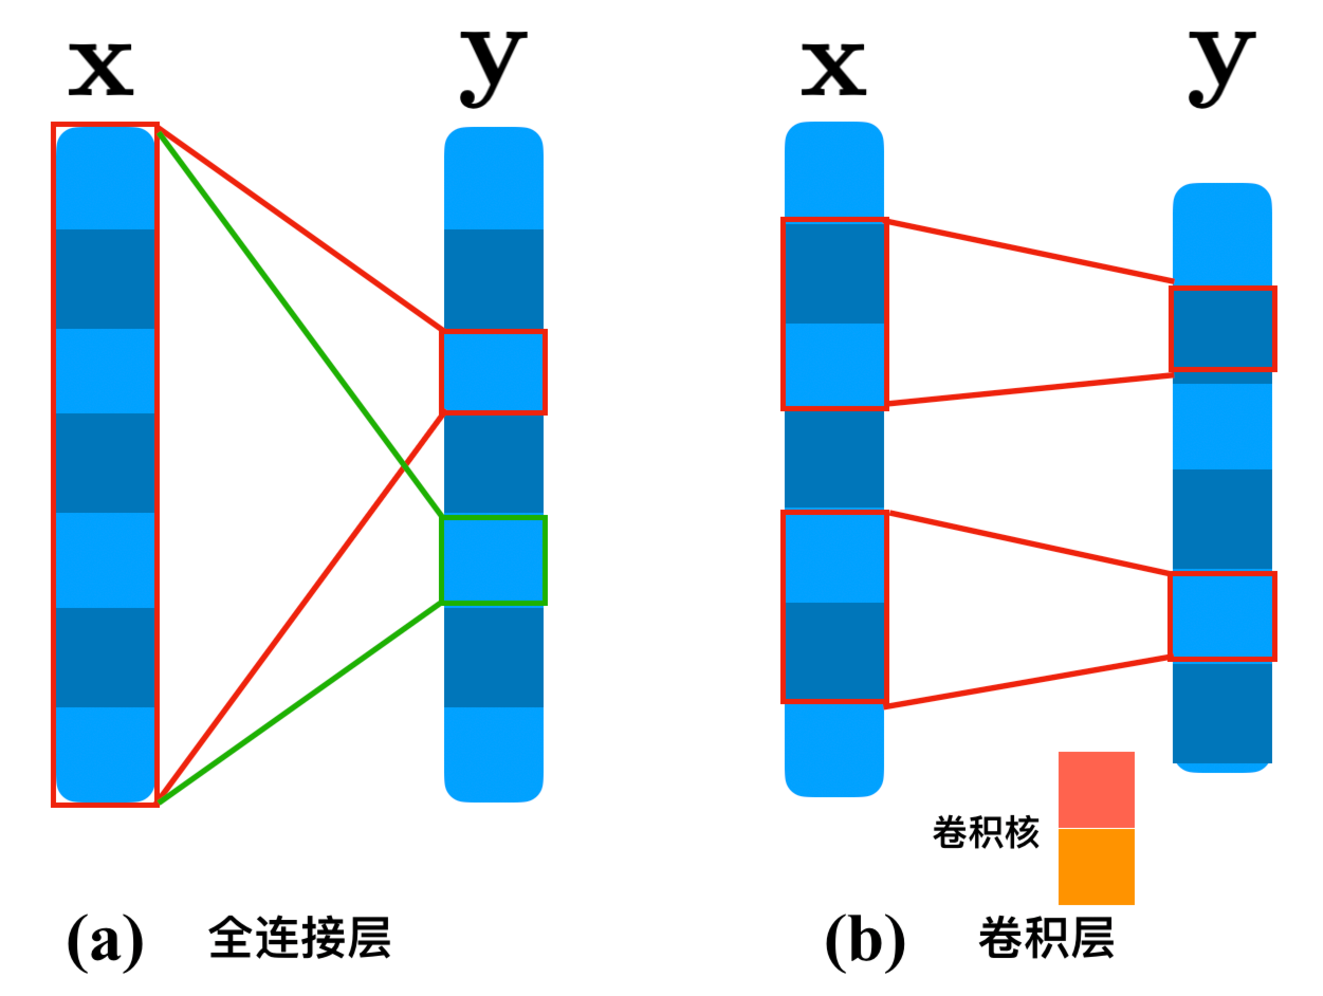
\includegraphics[width=0.8\columnwidth]{chap5_topoml/sketch}
\caption{
(a) 全连接层示意图;
(b) 卷积层示意图。}
\label{fig:sketch}
\end{figure}
\section{神经网络简介}
本节我们对神经网络这一机器学习\cite{prmlbook}中的重要算法进行简单介绍。当我们希望机器进行某项基本的任务,我们希望的是机器从我们输入的信息$\mathbf{x}$给出回复$\mathbf{y}$。例如,如果我们希望机器区分经典Ising系统的铁磁相与顺磁相,我们的输入$\mathbf{x}$便是某次实验测得的系统自旋构型$\mathbf{x}={0,0,0,1,1,0...}$,其中$0$代表自旋朝下,$1$代表自旋朝上。基于我们的输入,机器应当输出$y=0$或$1$,代表系统处在顺磁或铁磁态。从这一任务抽象出的数学问题,便是我们希望机器习得从$\mathbf{x}$到$\mathbf{y}$的某个复杂函数$\mathbf{y}=f(\mathbf{x})$。不同的机器学习算法,很多则是对应我们选取了不同的$f$的参数化形式。

神经网络也是一种函数$f$的参数化方式。在基础的神经网络中,我们假设复杂函数$f$可以通过简单函数的复合进行高效拟合:
\begin{align}
f(\mathbf{x})=f^n(...f^2(f^1(\mathbf{x},\mathbf{p}^1),\mathbf{p}^2)...,\mathbf{p}^n).
\end{align}
容易看到在这一函数中,每一个函数$f^i$的输出结果只依赖于上一结果$f^{i-1}$以及自身的参数$\mathbf{p}^i$,因此这一网络结构是单向的,我们称$f^i$为第$i$层。神经网络可以按照所选取的$f^i$形式不同分为全连接神经网络与卷积神经网络两种,其对应的核心函数$f^i$被称为全连接层与卷积层。下面两小节我们将分别对这两种层的结构进行介绍。


\subsection{全连接层与全连接神经网络}

\subsection{卷积层与卷积神经网络}



\section{二维陈数的深度学习}


\section{一维绕数的深度学习}

